Nella fase 4 vengono eseguite le seguenti attività:
\begin{itemize}
	\item normazione: modifiche alle \textit{Norme di progetto} secondo quanto segnalato alla Revisione dei requisiti. Si procede poi con il suo incremento;
	\item pianificazione della qualifica: modifiche al \textit{Piano di qualifica} secondo quanto segnalato alla Revisione di qualifica; Si procede poi con il suo incremento;
	\item pianificazione delle attività: modifiche al \textit{Piano di progetto} secondo quanto segnalato alla Revisione di qualifica;
	\item progettazione di dettaglio: incremento al \textit{Product Baseline} con secondo quanto segnalato alla Recisione di qualifica;
	\item codifica: codifica degli incrementi effettuati durante la progettazione;
	\item redazione manuali: incrementi al \textit{Manuale utente} e al \textit{Manuale sviluppatore} in base a quanto segnalato alla Revisione di qualifica;
	\item verifica: verifica degli incrementi effettuati;
	\item validazione e collaudo: vengono eseguiti i test di qualifica e il collaudo per il rilascio;
	\item preparazione alla presentazione;
	\item consegna del materiale in ingresso.
\end{itemize}

\begin{figure}[h]
	\centering
	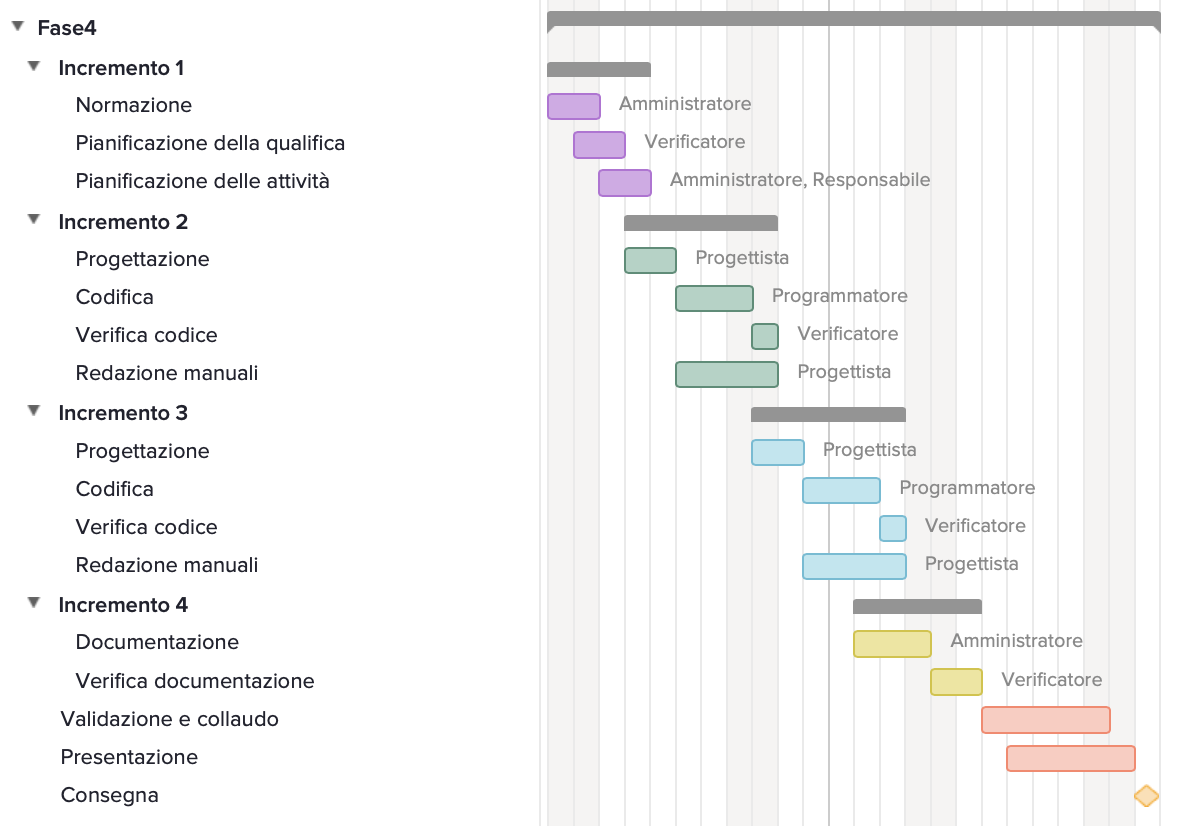
\includegraphics[scale=0.70]{images/fase4.png}
	\caption{Diagramma di Gantt riguardante la fase 4}
\end{figure}